\columnbreak
\part{Data Interpolation in 1D}
\setcounter{section}{0}

%Goal
\textbf{Goal:} Given $n$ data points $(t_i, y_i)$ and a finite-dimensional vector-space of functions $V$, reconstruct $f\in V$ such that $\forall i \quad f(t_i)=y_i$. \\
We denote with $\mathrm{I}_{\mathcal{T}}(\mathbf{y})$ the polynomial interpolation operator. \\

\Def[Interpol. as linear mapping] \\
For data points $(t_i, y_i) \quad i=0,\dots,n$
and $V$ spanned by basis functions $b_0,\dots b_m$ we have
$$
\mathbf{A} \mathbf{c}:=\left[\begin{array}{ccc}
b_{0}\left(t_{0}\right) & \ldots & b_{m}\left(t_{0}\right) \\
\vdots & & \vdots \\
b_{0}\left(t_{n}\right) & \ldots & b_{m}\left(t_{n}\right)
\end{array}\right]\left[\begin{array}{c}
c_{0} \\
\vdots \\
c_{m}
\end{array}\right]=\vy
$$
$\rightarrow$ The interpolant is uniquely solv. iff $m=n$\\
$\rightarrow$ The basis is \textbf{cardinal} if $b_{j}\left(t_{i}\right)=\delta_{i j}$

\section{Global Polynomial Interpol.}
In general global polynomial interpolation is not suitable due to potentially very high sensitivity. \\
We differentiate the following bases for polynomial representation. In any of these bases, evaluation is possible in $\BigO(n)$ by Horner-Like schemes that exploit associativity.

\Def[Monomial Basis]
$$ p_i(t) = t^i$$

\Def[Lagrange Basis]
$$L_{i}(t):=\prod_{j=0 \atop j \neq i}^{n} \frac{t-t_{j}}{t_{i}-t_{j}} = I_\mathcal{T}(\ve_{i+1})$$
$\rightarrow$ Cardinal Basis.

\Def[Newton Basis]
$$N_{i}(t):=\prod_{j=0}^{i-1} t-t_{j}$$

\sep

\Method[Multiple Evaluations] \\
$\rightarrow$ Barycentric Interpolation Formula. \\
Using precomputed weights in $\BigO(n^2)$ it achieves $\BigO(N n)$ to evaluate $N$ points.

\Method[Single Point Evaluation] \\
$\rightarrow$ Aitken-Neville scheme. \\
Evaluation in $\BigO(n^2)$ but addPoint in $\BigO(n)$.

\Method[Newton Interpolation] \\
$\rightarrow$ Coefficients in $\BigO(n^2)$, Evaluation in $\BigO(n)$ and Adding-a-Node in $\BigO(n)$. \\
Coefficients are computed with the \textit{Divided Differences} method, which is based on the following:
$$
a_{\ell, m}=\frac{a_{\ell+1, m}-a_{\ell, m-1}}{t_{m}-t_{\ell}}
$$
where $a_{\ell, m}$ denotes the leading coefficient of the the polynomial interpolating points $l \dots m$

\sep
\Method[Extrapolation] \\

\section{Shape-Preserving Interpol.}

\Def[Shape preserving] \\
positive data $\longrightarrow$ positive interpolant. \\
monotonic data $\longrightarrow$ monotonic interpolant.\\
convex data $\longrightarrow$ convex interpolant. \\

\Method[Piecewise linear Interpol.] \\
$\rightarrow$ locally shape preserving \\
Tent functions make a cardinal basis:
\begin{center}
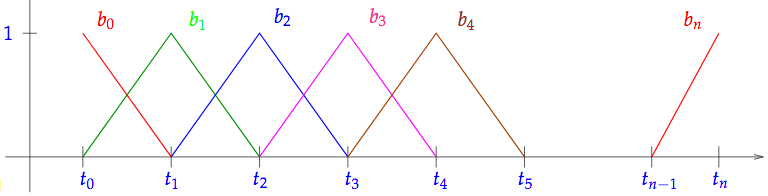
\includegraphics[height=25px, width=\columnwidth,]{5_tent.png}
\end{center}

\Method[Cubic Hermite Interpol.] \\
$\rightarrow$ f $\in C^{1}\left(\left[t_{0}, t_{n}\right]\right)$ \\
Idea: Interpolate each interval as cubic polynomial but edge points have to match, and derivatives on edges have to match. But we have to decide what we want derivates to be at edge:
\begin{itemize}
	\item Linear: (weighted mean of adjacent derivatives) -> No Preservation of monotonicity
	\item Pchip: Since slope must be zero at boundary in some cases -> Loss of linearity
\end{itemize}

\section{Splines}
Instead of fixing the boundary slopes, we add additional continuity constraints. The interpolating function $f$ is then in the Spline Space.\\

\Def[Spline Space] 
$${\scriptstyle
\mathcal{S}_{d, \mathcal{M}}:=\left\{s \in C^{d-1}(I): s_{j}:=s_{\mid\left[t_{j-1}, t_{j}\right]} \in \mathcal{P}_{d} \forall j=1, \ldots, n\right\}}
$$
$\mathcal{S}_{d, \mathcal{M}}$ is the space of piecewise polynomial functions in $C^{d-1}$. One can easily see that $$
\operatorname{dim} \mathcal{S}_{d, \mathcal{M}}=n+d
$$

\Method[Cubic Spline Interpolation] The cubic spline interpolant is a function $s \in \mathcal{S}_{3, \mathcal{M}}$ that complies with the $n+1$ interpolation conditions. Note that we still have 2 degrees of freedom, this leads to the following flavours:
\begin{itemize}
	\item natural: $s^{\prime}\left(t_{0}\right)=0, s^{\prime}\left(t_{n}\right)=0$
	\item periodic: $s^{\prime}\left(t_{0}\right)=s^{\prime}\left(t_{n}\right), s^{\prime\prime}\left(t_{0}\right)=s^{\prime\prime}\left(t_{n}\right)$
	\item complete: $s^{\prime}\left(t_{0}\right)=c_{0}, s^{\prime}\left(t_{n}\right)=c_{n}$
\end{itemize}
The resulting functions is in $C^2$, weakly-local and not strictly shape preserving.

\section{Trigonometric Interpol.}
bla

\section{Least Squares Data Fitting}
\textbf{Goal:} Given $m$ data points $(t_i, y_i)$ and a set of functions $V$, find a continuous function $f\in V$ such that
$$
f \in \underset{\mathbf{g} \in S}{\operatorname{argmin}}\|\textbf{g}(t_i)-y_i\|_{2}^{2}
$$
We focus on \textbf{linear} data fitting, i.o.w. let $V$ be an $n$-dimensional vector space spanned by functions $b_1(t), \dots, b_n(t)$. We look for coefficients 
$$[x_1,\dots,x_n]^T=\underset{\mathbf{z} \in \mathbb{R}^{n}}{\operatorname{argmin}} \sum_{i=1}^{m}\left|\sum_{j=1}^{n}(\mathbf{z})_{j} b_{j}\left(t_{i}\right)-y_{i}\right|^{2}$$

\Theorem[Linear Data Fitting Solution] \\
The solution to the linear least squares fitting problem is the least squares solution of the system
$$
\left[\begin{array}{ccc}
b_{1}\left(t_{1}\right) & \ldots & b_{n}\left(t_{1}\right) \\
\vdots & & \vdots \\
b_{1}\left(t_{m}\right) & \ldots & b_{n}\left(t_{m}\right)
\end{array}\right]
\vx = \left[\begin{array}{c}
y_{1} \\
\vdots \\
y_{m}
\end{array}\right]
$$

\Method[Regularization] We can punish large oscillations by introducing a regularization term:
$$
f \in \underset{g \in V}{\operatorname{argmin}}\left\{\sum_{i=0}^{n}\left|g\left(t_{i}\right)-y_{i}\right|^{2}+\alpha \int_{a}^{b}\left|g^{\prime \prime}(t)\right|^{2} \mathrm{~d} t\right\}
$$